%!TeX program = xelatex
\documentclass{article}
\usepackage{papers}

%%-------------------------------正文开始---------------------------%%
\begin{document}

%%-----------------------封面--------------------%%
\maketitle

%%------------------摘要-------------%%
\begin{abstract}
在本次测试中,openGauss 数据库在 RISC-V 平台上表现出了初步的可用性。我们在 Milk-V Pioneer Box 和 Sipeed LicheePi 4A 两个典型平台上进行了测试。结果表明,Milk-V Pioneer Box 能够稳定运行 openGauss,并支持本地及远程连接,表现出较好的用户体验。然而,Sipeed LicheePi 4A 由于硬件性能的限制,无法正常启动 openGauss 服务。测试采用 openEuler 24.03 LTS 系统,并手动编译 openGauss 6.0.0 版本。功能测试涵盖了基本的数据库操作,确认了 openGauss 的基本功能正常可用。在性能测试中,通过 sysbench 工具,我们评估了数据库在多线程读写和只读场景下的性能。虽然 Milk-V Pioneer Box 在只读负载下表现相对较好,但整体性能仍不及 x86\_64 平台。本次测试为 openGauss 在 RISC-V 平台的进一步优化和支持提供了参考。未来的优化方向包括提升在低性能硬件平台上的表现,以及增加对更多操作系统和环境的支持,以提升其广泛性和竞争力。
\end{abstract}

\thispagestyle{empty} % 首页不显示页码

%%--------------------------目录页------------------------%%
\newpage
\tableofcontents

%%------------------------正文页从这里开始-------------------%
\newpage

\section{简介}

\subsection{软件说明}
openGauss 是一个免费的开源关系型数据库管理系统,主要由华为开发和维护。它是一个广泛使用的代码库,为企业级应用提供了高性能、高可用性和高安全性的数据库解决方案。

\subsection{测试目的}
本次测试旨在验证 openGauss 在 RISC-V 平台上的可用性,特别是在 Milk-V Pioneer Box 和 Sipeed LicheePi 4A 两个典型平台上的表现。本报告通过手动测试的方法,从目前的平台兼容性及用户的日常使用体验两个角度评估了 openGauss 当前在 RISC-V 平台上的可用性,并给出了定性和定量的结论,为其未来进一步的优化和支持提供参考。

\subsection{测试概述}
在本次测试中,我们评估了 openGauss 数据库在 RISC-V 平台上的可靠性和性能表现,尤其是在 Milk-V Pioneer Box 和 Sipeed LicheePi 4A 这两个平台上。Milk-V Pioneer Box 具备较强的处理能力,可以成功安装和运行 openGauss 数据库,并支持本地和远程连接。
测试使用了 openEuler 24.03 LTS 系统并手动编译 openGauss 6.0.0 版本。在功能测试部分,我们首先通过 gsql 和 dbeaver 工具验证了基本的数据库操作,包括用户和数据库的创建、基本的表操作等。在性能测试中,我们使用 sysbench 工具进行了读写和只读性能测试。为了进行比较,也在 x86\_64 平台上进行同样的测试。

\subsection{测试总结}
目前 openGauss 在 riscv 上仅支持使用 openEuler 系统进行编译与安装,licheepi 4a 因为性能不足而无法启动 openGauss 服务,
Pioneer Box 可以正常本地和远程连接与使用.

使用 sysbench 在 Pioneer Box 上性能测试结果如下:

\textbf{SQL statistics}

\begin{itemize}
    \item rw: oltp 测试,包含读写 
    \item r:select 测试,仅读
\end{itemize}

\begin{table}[h]
\centering
\begin{tabular}{|l|r|r|r|r|r|r|r|r|r|r|}
\hline
Platform & read & write & other & total & transactions & transactions/s & queries & queries/s & ignored errors & reconnects \\
\hline
SG2042 @ 10 Threads rw & 278796 & 79654 & 39828 & 398278 & 11913 & 331.56 & 398278 & 6631.51 & 1 & 0 \\
SG2042 @ 64 Threads rw & 952280 & 272041 & 136057 & 1360378 & 68009 & 1128.35 & 1360378 & 22750.22 & 11 & 0 \\
SG2042 @ 64 Threads r  & 1851630 & 0      & 0      & 1851630 & 1851630 & 30766.50 & 1851630 & 30766.50 & 0 & 0 \\
X86\_64 @ 10 Threads rw & 584472 & 166989 & 83497 & 834958 & 41747 & 695.69 & 834958 & 13914.18 & 1 & 0 \\
\hline
\end{tabular}
\end{table}

\textbf{Latency}

\begin{table}[h]
\centering
\begin{tabular}{|l|r|r|r|r|r|}
\hline
Platform & min & avg & max & 95th percentile & sum \\
\hline
SG2042 @ 10 Threads rw & 25.62 & 30.13 & 99.91 & 33.72 & 599938.70 \\
SG2042 @ 64 Threads rw & 38.63 & 56.49 & 421.75 & 70.55 & 3842023.49 \\
SG2042 @ 64 Threads rw & 1.12 & 2.06 & 353.15 & 3.30 & 3822093.08 \\
X86\_64 @ 10 Threads rw & 5.23 & 14.37 & 1569.33 & 21.50 & 599913.47 \\
\hline
\end{tabular}
\end{table}


\textbf{Threads fairness}

\begin{table}[h]
\centering
\begin{tabular}{|l|r|r|r|r|}
\hline
Platform & events avg & events stddev & execution time avg & execution time stddev \\
\hline
SG2042 @ 10 Threads rw & 1991.3000 & 32.68 & 59.9939 & 0.01 \\
SG2042 @ 64 Threads rw & 1062.6406 & 24.58 & 60.0316 & 0.03 \\
SG2042 @ 64 Threads r & 28931.7188 & 1217.10 & 59.7202 & 0.03 \\
X86\_64 @ 10 Threads rw & 4174.7000 & 12.74 & 59.9913 & 0.00 \\
\hline
\end{tabular}
\end{table}

\section{环境说明}

\subsection{硬件环境}
本次测试主要在 Milk-V Pioneer Box 和 Sipeed LicheePi 4A 上进行,机器硬件配置为:

Milk-V Pioneer Box:
\begin{itemize}
    \item CPU: SG2042 64 Core C920@2.0GHz
    \item RAM: 4 channel 3200Hz 128GB DDR4 SODIMM (32GB * 4)
    \item SSD: PCIe 3.0 x 4 1TB
    \item GPU: AMD R5 230
\end{itemize}

Sipeed LicheePi 4A:
\begin{itemize}
    \item CPU: TH1520, RISC-V 2.0G C910 x4
    \item RAM: 16 GB 64bit LPDDR4X-3733
    \item Storage: 128 GB eMMC
\end{itemize}

x86\_64:
\begin{itemize}
    \item CPU: Xeon Gold 5215L CPU @ 2.50GHz, 10*vCPU (Proxmox VE 8.0 虚拟化环境)
    \item RAM: 8 GiB
\end{itemize}

\subsection{软件环境}
本次测试涵盖的系统版本和 openGauss 版本如下:

\begin{itemize}
    \item \href{https://www.openeuler.org/zh/download/?version=openEuler%2024.03%20LTS}{openEuler} 24.03 LTS
    \item \href{https://gitee.com/opengauss/riscv}{openGauss} 6.0.0
\end{itemize}

\subsection{测试环境搭建}

\subsubsection{安装 openEuler}

\paragraph{Sipeed LicheePi 4A}

从 \href{https://www.openeuler.org/zh/download/?version=openEuler%2024.03%20LTS}{官网} 下载镜像:

选择 `RISC-V - 嵌入式 - lpi4a`。

使用 `fastboot` 刷写镜像到板载 eMMC

由于 LPi4A 默认的 USB VID/PID 通常不在默认 udev 规则内,在 Linux 下烧写时可能需要在 `fastboot` 前添加 `sudo`。

按住板上的 \textbf{BOOT} 按键不放,然后插入 USB-C 线缆上电(线缆另一头接 PC),即可进入 USB 烧录模式。

在 Windows 下使用设备管理器查看,会出现 `USB download gadget` 设备。

在 Linux 下,使用 `lsusb` 查看设备,会显示以下设备:`ID 2345:7654 T-HEAD USB download gadget`。

使用如下指令刷写镜像。

\begin{verbatim}
fastboot flash ram u-boot-with-spl-lpi4a-16g.bin
fastboot reboot
# 稍等几秒,等待开发板重启后重新连接至电脑
fastboot flash uboot u-boot-with-spl-lpi4a-16g.bin
fastboot flash boot openEuler-24.03-LTS-riscv64-lpi4a-base-boot.ext4
fastboot flash root openEuler-24.03-LTS-riscv64-lpi4a-base-root.ext4
\end{verbatim}

\paragraph{Milk-V Pioneer Box}

下载\href{https://mirrors.hust.edu.cn/openeuler/openEuler-24.03-LTS/embedded_img/riscv64/SG2042/openEuler-24.03-LTS-riscv64-sg2042.img.zip}{系统镜像},解压,使用 `dd` 烧录至 NVMe 硬盘。
下载\href{https://mirrors.hust.edu.cn/openeuler/openEuler-24.03-LTS/embedded_img/riscv64/SG2042/sg2042_firmware_linuxboot.img.zip}{固件},解压,使用 `dd` 烧录至 microSD 卡。

请将下面的 `/dev/sda` `/dev/sdb` 替换成实际使用的硬盘和存储卡位置。

\begin{verbatim}
unzip openEuler-24.03-LTS-riscv64-sg2042.img.zip
sudo wipefs -af /dev/sda
sudo dd if=openEuler-24.03-LTS-riscv64-sg2042.img of=/dev/sda bs=1M status=progress
sudo eject /dev/sda
unzip sg2042_firmware_linuxboot.img.zip
sudo dd if=sg2042_firmware_linuxboot.img of=/dev/sdb bs=1M status=progress
\end{verbatim}
将存储卡和硬盘插入系统上电开机。

\subsubsection{安装 openGauss 数据库}

因为\href{https://opengauss.org/zh/download/}{官网提供的下载中}没有 riscv 架构的,所以需要手动构建并安装 opengauss 数据库

此文档针对 riscv 平台编写,在其他平台下使用请自行配置 qemu

\paragraph{编译}

使用 openEuler 容器编译可参考 \href{https://github.com/QA-Team-lo/dbtest/blob/main/opengauss/install.md}{此链接}

以下使用 Pioneer Box 裸机编译:

下载源码

\begin{verbatim}
su 
mkdir /root/rpmbuild
cd /root/rpmbuild
git clone https://gitee.com/opengauss/riscv SOURCES
cd SOURCES
\end{verbatim}

配置编译环境

\begin{verbatim}
# 安装必要工具
dnf install -y rpm-build rpmdevtools dnf-plugins-core
# 安装编译依赖
yum-builddep -y opengauss-server.spec
# 下载源码
spectool -g opengauss-server.spec
\end{verbatim}

编译 rpm 包

\begin{verbatim}
rpmbuild -ba opengauss-server.spec
\end{verbatim}

\paragraph{安装}
等待一段时间,编译完成后,安装

\begin{verbatim}
cd ../RPMS/riscv64/
dnf install -y opengauss-server-6.0.0-1.riscv64.rpm
\end{verbatim}

\paragraph{初始化 \& 启动}

\begin{verbatim}
systemctl enable --now opengauss-server
\end{verbatim}

\subsection{功能测试}

在 PostgreSQL 中创建数据库和用户:
\begin{verbatim}
# 切换至 opengauss 用户
su opengauss

# 连接数据库
gsql -d postgres
\end{verbatim}

当 gsql 连接数据库成功后,在 gsql 交互界面中输入
\begin{verbatim}
-- 修改默认用户密码
alter role "opengauss" password "openGauss@2024";

-- 创建用户
CREATE USER testuser WITH PASSWORD 'openEuler12#$';

-- 创建数据库
CREATE DATABASE testdb owner testuser;
\end{verbatim}


修改 opengauss 配置文件
\begin{verbatim}
vim /var/lib/opengauss/data/postgresql.conf
# 配置 listen_addresses = '*'
# 配置 password_encryption_type = 1

vim /var/lib/opengauss/data/pg_hba.conf
# 末尾增加: 
# host     all          testuser           0.0.0.0/0               md5

gs_ctl -D $HOME/data reload
# reload 后即可生效
\end{verbatim}

\subsubsection{性能测试}

安装 sysbench
\begin{verbatim}
sudo dnf install sysbench
\end{verbatim}

修改 opengauss 配置文件
\begin{verbatim}
vim /var/lib/opengauss/data/postgresql.conf
# 配置 listen_addresses = '*'
# 配置 password_encryption_type = 1

gs_ctl -D $HOME/data reload
# reload 后即可生效
\end{verbatim}

在 openGauss 中创建数据库和用户(在修改密码规则后必须新建用户或修改密码才能使用)
\begin{verbatim}
su - opengauss

gsql -d postgres

CREATE USER testuser WITH PASSWORD 'openEuler12#$';

CREATE DATABASE testdb owner testuser;
\end{verbatim}

授予权限用于测试

\begin{verbatim}
[opengauss@openeuler-riscv64 openeuler]$ gsql -d postgres
gsql ((openGauss-lite 6.0.0 build ) compiled at 2024-11-22 20:54:23 commit 0 last mr  release)
Non-SSL connection (SSL connection is recommended when requiring high-security)
Type "help" for help.

openGauss=# GRANT ALL ON SCHEMA public TO testuser;
GRANT
openGauss=# GRANT ALL PRIVILEGES TO testuser; 
ALTER ROLE
\end{verbatim}


\section{测试内容}

\subsection{手动测试}

\subsubsection{本地测试}
使用 `gsql -U testuser -d testdb` 连接数据库,创建表,并作简单的增删查操作
\begin{verbatim}
create table phonebook (
    id serial primary key,
    name varchar(20),
    phone varchar(20)
);

insert into phonebook (name, phone) values ('工商银行', '95588');
insert into phonebook (name, phone) values ('招商银行', '95555');
insert into phonebook (name, phone) values ('农业银行', '95599');

insert into phonebook (name, phone) values ('邮政快递', '11183');
insert into phonebook (name, phone) values ('顺丰快递', '95338');
insert into phonebook (name, phone) values ('京东物流', '95311');

select * from phonebook where name like '%银行';
select count(*) from phonebook;
delete from phonebook where name = '农业银行';
select * from phonebook;
\end{verbatim}

\subsubsection{远程测试}

下载 \href{https://opengauss.org/zh/download/}{JDBC\_6.0.0} 数据库驱动并解压

启动 Dbeaver,并选择菜单->数据库->驱动管理器,在弹出对话框中,选择新建

\begin{center}
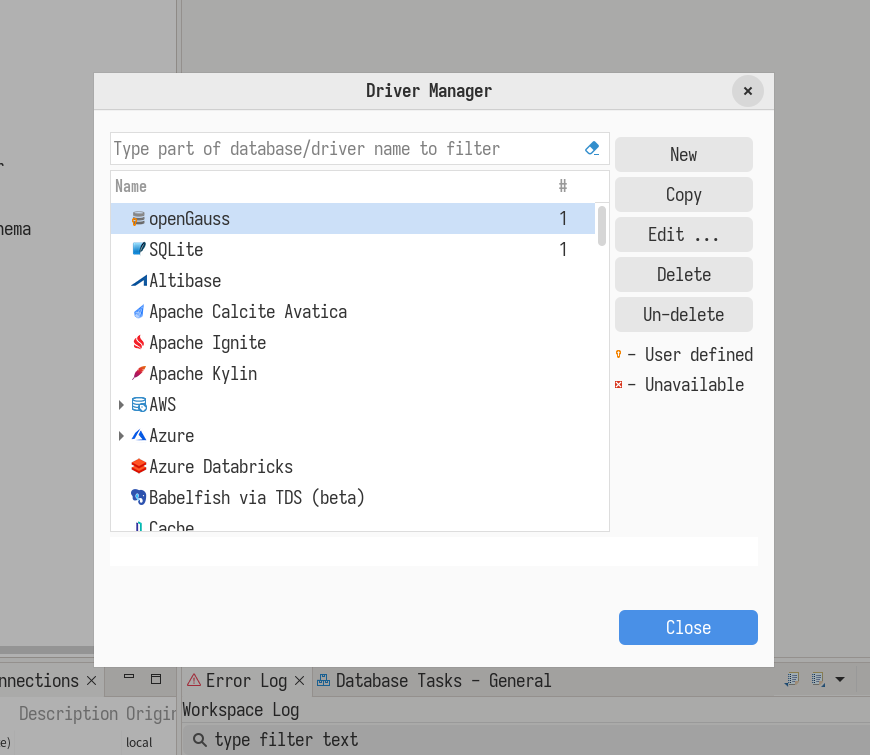
\includegraphics[width=9cm]{./image/1.png}
\end{center}

填写新建驱动名称->选择 JDBC 驱动文件,添加解压出来的`opengauss-jdbc-6.0.0.jar`->选择 JDBC Driver 类

\begin{center}
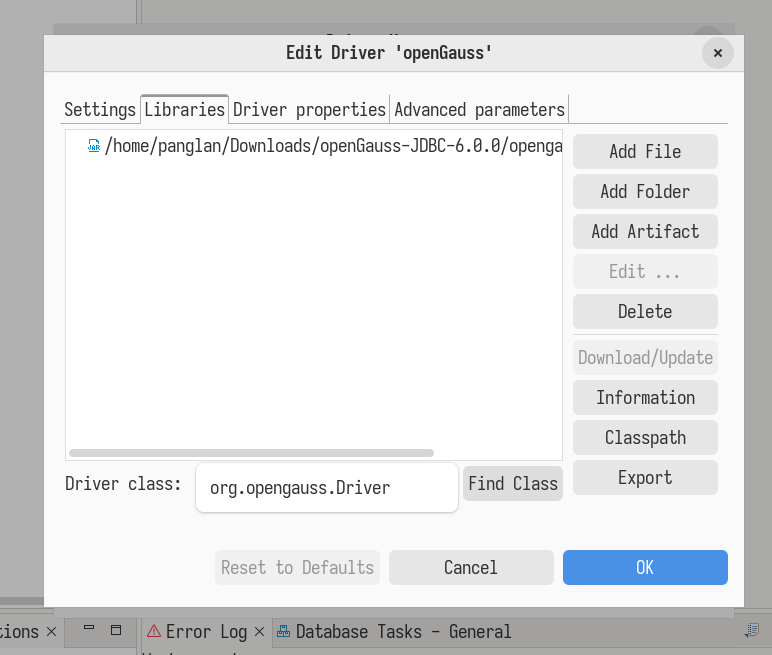
\includegraphics[width=9cm]{./image/3.png}
\end{center}

填写 URL 模板,值为:`jdbc:opengauss://{host}:{port}/{database}`,勾选嵌入,其他复选框不选择,然后确认,添加驱动即完成

\begin{center}
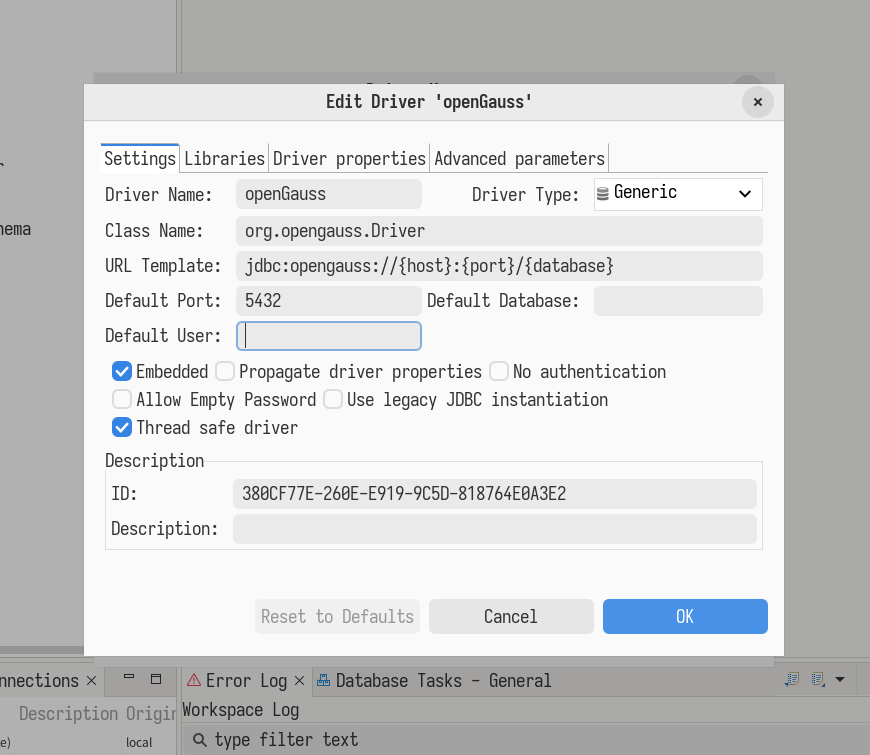
\includegraphics[width=9cm]{./image/2.png}
\end{center}

选择菜单->数据库->新建连接,在弹出的框中搜索上一步中新建的 JDBC 驱动名,选择后点击下一步,如下图示

\begin{center}
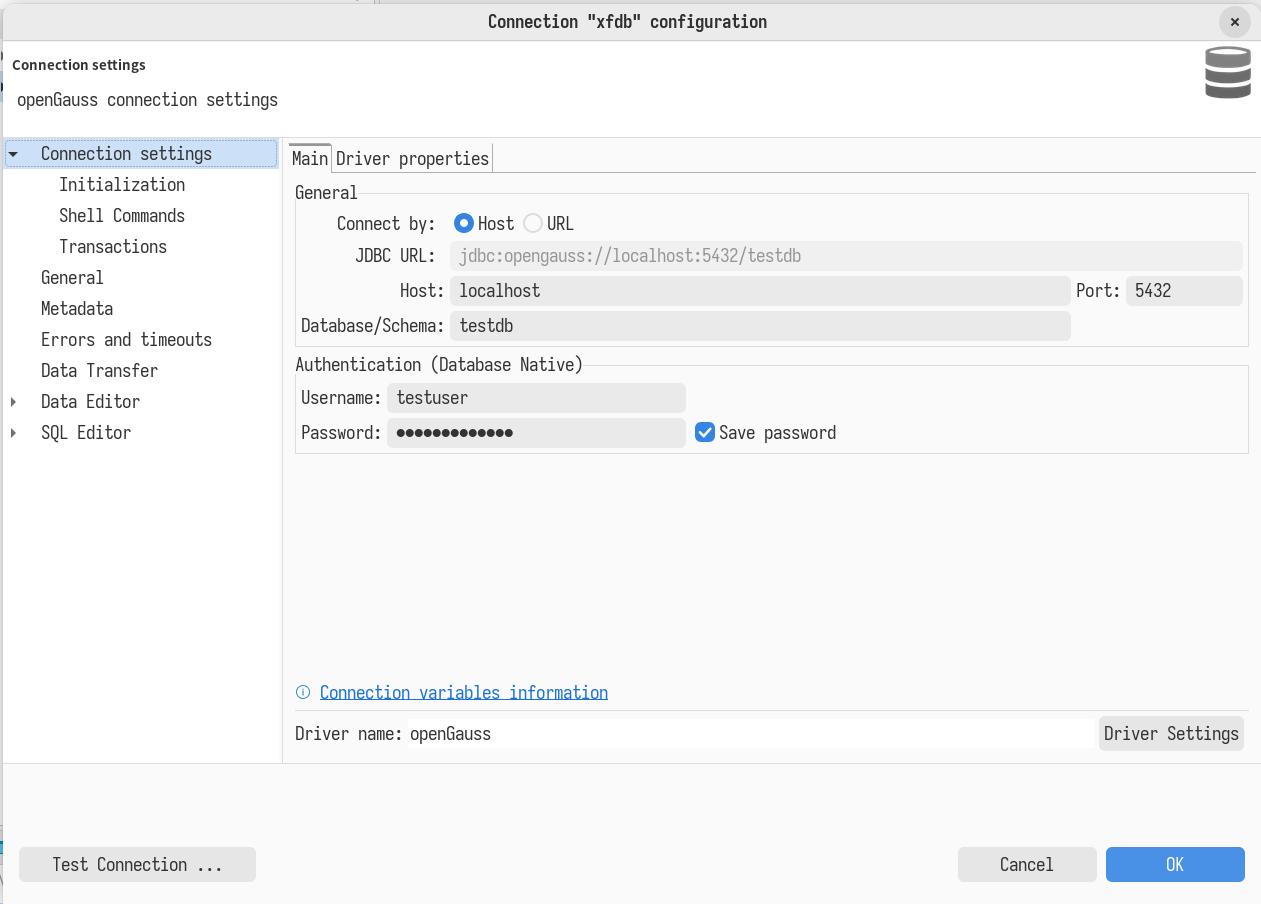
\includegraphics[width=9cm]{./image/4.png}
\end{center}

在弹出框中填写 openGauss 主机地址、端口、将要连接的数据库以及认证用户名和密码,点击测试链接验证是否可正确连接

\begin{center}
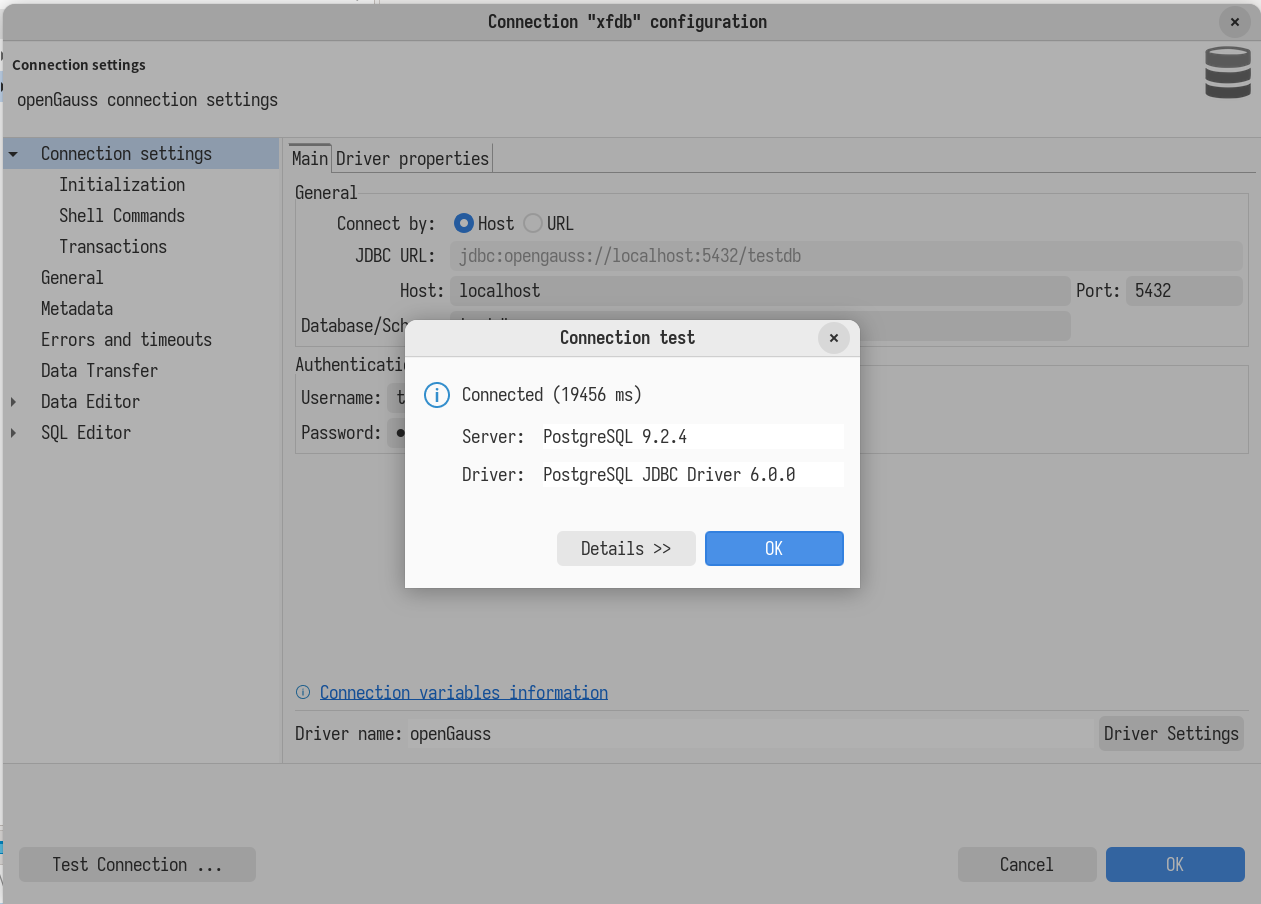
\includegraphics[width=9cm]{./image/5.png}
\end{center}


\subsection{性能测试}

初始化数据库
\begin{verbatim}
sysbench --db-driver=pgsql --oltp-table-size=100000 --oltp-tables-count=24 --threads=1 --pgsql-host=127.0.0.1 --pgsql-port=5432 --pgsql-user=testuser --pgsql-password=openEuler12#$ --pgsql-db=testdb  /usr/share/sysbench/tests/include/oltp_legacy/parallel_prepare.lua run
\end{verbatim}

使用下列命令验证生成的数据
\begin{verbatim}
[opengauss@openeuler-riscv64 openeuler]$ gsql -U testuser -d testdb
Password for user testuser: 
gsql ((openGauss-lite 6.0.0 build ) compiled at 2024-11-22 20:54:23 commit 0 last mr  release)
Non-SSL connection (SSL connection is recommended when requiring high-security)
Type "help" for help.

testdb=> \dt
                            List of relations
 Schema |   Name   | Type  |  Owner   |             Storage              
--------+----------+-------+----------+----------------------------------
 public | sbtest1  | table | testuser | {orientation=row,compression=no}
 public | sbtest10 | table | testuser | {orientation=row,compression=no}
 public | sbtest11 | table | testuser | {orientation=row,compression=no}
 public | sbtest12 | table | testuser | {orientation=row,compression=no}
 public | sbtest13 | table | testuser | {orientation=row,compression=no}
 public | sbtest14 | table | testuser | {orientation=row,compression=no}
 public | sbtest15 | table | testuser | {orientation=row,compression=no}
 public | sbtest16 | table | testuser | {orientation=row,compression=no}
 public | sbtest17 | table | testuser | {orientation=row,compression=no}
 public | sbtest18 | table | testuser | {orientation=row,compression=no}
 public | sbtest19 | table | testuser | {orientation=row,compression=no}
 public | sbtest2  | table | testuser | {orientation=row,compression=no}
 public | sbtest20 | table | testuser | {orientation=row,compression=no}
 public | sbtest21 | table | testuser | {orientation=row,compression=no}
 public | sbtest22 | table | testuser | {orientation=row,compression=no}
 public | sbtest23 | table | testuser | {orientation=row,compression=no}
 public | sbtest24 | table | testuser | {orientation=row,compression=no}
 public | sbtest3  | table | testuser | {orientation=row,compression=no}
 public | sbtest4  | table | testuser | {orientation=row,compression=no}
 public | sbtest5  | table | testuser | {orientation=row,compression=no}
 public | sbtest6  | table | testuser | {orientation=row,compression=no}
 public | sbtest7  | table | testuser | {orientation=row,compression=no}
 public | sbtest8  | table | testuser | {orientation=row,compression=no}
 public | sbtest9  | table | testuser | {orientation=row,compression=no}
(24 rows)

testdb=> \d sbtest1
                             Table "public.sbtest1"
 Column |      Type      |                      Modifiers                       
--------+----------------+------------------------------------------------------
 id     | integer        | not null default nextval('sbtest1_id_seq'::regclass)
 k      | integer        | not null default 0
 c      | character(120) | not null default NULL::bpchar
 pad    | character(60)  | not null default NULL::bpchar
Indexes:
    "sbtest1_pkey" PRIMARY KEY, btree (id) TABLESPACE pg_default
    "k_1" btree (k) TABLESPACE pg_default

testdb=> \q
\end{verbatim}


执行读/写测试
\begin{verbatim}
sysbench --db-driver=pgsql --report-interval=2 --oltp-table-size=100000 --oltp-tables-count=24 --threads=64 --time=60 --pgsql-host=127.0.0.1 --pgsql-port=5432 --pgsql-user=testuser --pgsql-password=openEuler12#$ --pgsql-db=testdb /usr/share/sysbench/tests/include/oltp_legacy/oltp.lua run
\end{verbatim}
上述命令将从名为 /usr/share/sysbench/tests/include/oltp\_legacy/oltp.lua 的 LUA 脚本生成 OLTP 工作负载,针对主服务器上 24 个表的 100,000 行(具有 64 个工作线程)持续 60 秒)。每 2 秒,sysbench 将报告中间统计信息(\verb!--report-interval=2!)。

执行只读测试
\begin{verbatim}
sysbench --db-driver=pgsql --report-interval=2 --oltp-table-size=100000 --oltp-tables-count=24 --threads=64 --time=60 --pgsql-host=127.0.0.1 --pgsql-port=5432 --pgsql-user=testuser --pgsql-password=openEuler12#$ --pgsql-db=testdb /usr/share/sysbench/tests/include/oltp_legacy/select.lua run
\end{verbatim}

清理测试数据
\begin{verbatim}
sysbench --db-driver=pgsql --report-interval=2 --oltp-table-size=100000 --oltp-tables-count=24 --threads=64 --time=60 --pgsql-host=127.0.0.1 --pgsql-port=5432 --pgsql-user=testuser --pgsql-password=openEuler12#$ --pgsql-db=testdb /usr/share/sysbench/tests/include/oltp_legacy/select.lua cleanup
\end{verbatim}


\section{测试结果}

\subsection{功能测试}
licheepi 4a 由于性能较弱,在启动 openGauss 服务时超时,而 Pioneer Box 可以正常进行本地和远程连接

使用 dbeaver 远程连接 openGauss 数据库结果如图所示:

\begin{center}
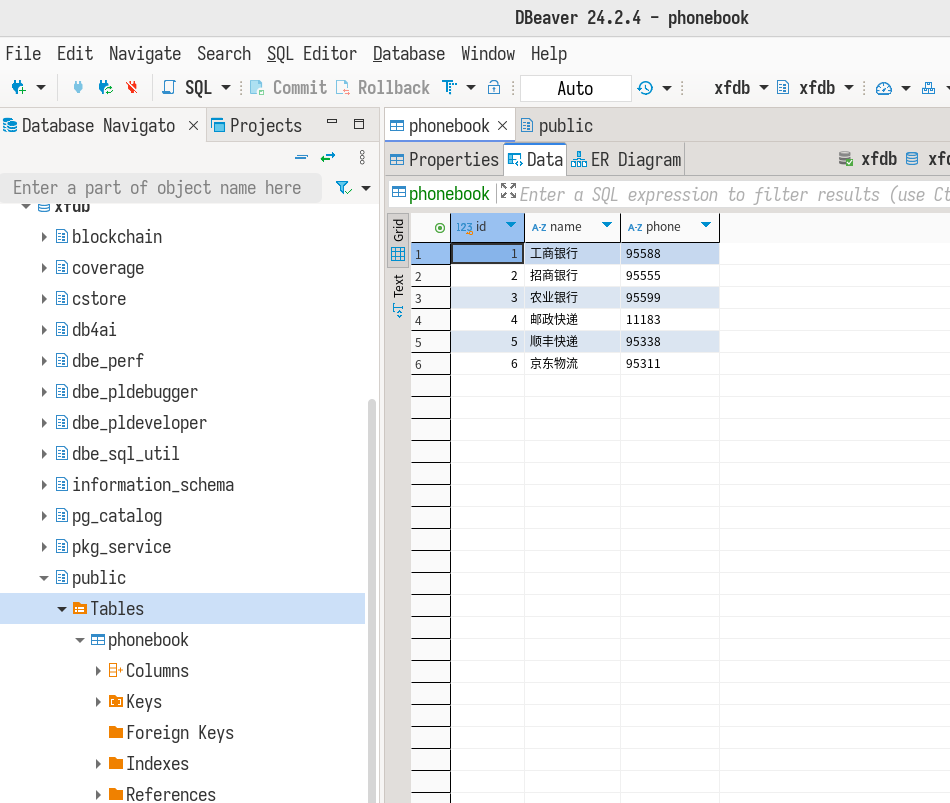
\includegraphics[width=9cm]{./image/6.png}
\end{center}

\subsection{性能测试}

详细结果参见 \href{https://github.com/QA-Team-lo/dbtest/tree/main/opengauss/logs}{logs} 目录或附录。

性能对比

\textbf{SQL statistics}

\begin{itemize}
    \item rw: oltp 测试,包含读写 
    \item r:select 测试,仅读
\end{itemize}

\begin{table}[h]
\centering
\begin{tabular}{|l|r|r|r|r|r|r|r|r|r|r|}
\hline
Platform & read & write & other & total & transactions & transactions/s & queries & queries/s & ignored errors & reconnects \\
\hline
SG2042 @ 10 Threads rw & 278796 & 79654 & 39828 & 398278 & 11913 & 331.56 & 398278 & 6631.51 & 1 & 0 \\
SG2042 @ 64 Threads rw & 952280 & 272041 & 136057 & 1360378 & 68009 & 1128.35 & 1360378 & 22750.22 & 11 & 0 \\
SG2042 @ 64 Threads r  & 1851630 & 0      & 0      & 1851630 & 1851630 & 30766.50 & 1851630 & 30766.50 & 0 & 0 \\
X86\_64 @ 10 Threads rw & 584472 & 166989 & 83497 & 834958 & 41747 & 695.69 & 834958 & 13914.18 & 1 & 0 \\
\hline
\end{tabular}
\end{table}

\textbf{Latency}

\begin{table}[h]
\centering
\begin{tabular}{|l|r|r|r|r|r|}
\hline
Platform & min & avg & max & 95th percentile & sum \\
\hline
SG2042 @ 10 Threads rw & 25.62 & 30.13 & 99.91 & 33.72 & 599938.70 \\
SG2042 @ 64 Threads rw & 38.63 & 56.49 & 421.75 & 70.55 & 3842023.49 \\
SG2042 @ 64 Threads rw & 1.12 & 2.06 & 353.15 & 3.30 & 3822093.08 \\
X86\_64 @ 10 Threads rw & 5.23 & 14.37 & 1569.33 & 21.50 & 599913.47 \\
\hline
\end{tabular}
\end{table}

\textbf{Threads fairness}

\begin{table}[h]
\centering
\begin{tabular}{|l|r|r|r|r|}
\hline
Platform & events avg & events stddev & execution time avg & execution time stddev \\
\hline
SG2042 @ 10 Threads rw & 1991.3000 & 32.68 & 59.9939 & 0.01 \\
SG2042 @ 64 Threads rw & 1062.6406 & 24.58 & 60.0316 & 0.03 \\
SG2042 @ 64 Threads r & 28931.7188 & 1217.10 & 59.7202 & 0.03 \\
X86\_64 @ 10 Threads rw & 4174.7000 & 12.74 & 59.9913 & 0.00 \\
\hline
\end{tabular}
\end{table}

\subsection{已知问题}

时间所限,笔者暂时没有找到合适的测试机,文中所使用的 Openeuler X86\_64 机器运行在 Hdd 上,I/O 性能会有严重瓶颈。这可能会影响 Opengauss 的性能表现。

x86\_64 机器运行在 PVE 虚拟化环境下。通常来说,KVM 虚拟化会有性能损失,但不会很大。这也可能会影响性能表现。

此外,内存大小不同也可能影响性能。

\section{总结}

本次测试确认了 openGauss 在 RISC-V 平台上的初步可用性。在 Milk-V Pioneer Box 上,openGauss 能够稳定运行并提供良好的用户体验,而在性能更低的 Sipeed LicheePi 4A 上,由于硬件的限制,无法顺利启动服务。性能测试结果显示,在多线程操作下,Milk-V Pioneer Box 的性能与 x86\_64 平台相比仍有差距。具体来说,在读写混合负载下,x86_64 平台的事务和查询处理能力明显高于 Pioneer Box。

\newpage
\appendix

\section{附录}

\paragraph{SG2042 openEuler 2403 10 线程}

\begin{verbatim}
sysbench 1.0.20 (using system LuaJIT 2.1.ROLLING)

Running the test with following options:
Number of threads: 10
Report intermediate results every 2 second(s)
Initializing random number generator from current time

Initializing worker threads...

Threads started!

[ 2s ] thds: 10 tps: 309.76 qps: 6252.70 (r/w/o: 4385.71/1242.51/624.48) lat (ms,95%): 34.95 err/s: 0.00 reconn/s: 0.00
[ 4s ] thds: 10 tps: 332.75 qps: 6657.07 (r/w/o: 4660.05/1331.51/665.51) lat (ms,95%): 34.33 err/s: 0.00 reconn/s: 0.00
[ 6s ] thds: 10 tps: 324.53 qps: 6499.64 (r/w/o: 4552.45/1297.13/650.06) lat (ms,95%): 35.59 err/s: 0.50 reconn/s: 0.00
[ 8s ] thds: 10 tps: 332.51 qps: 6644.63 (r/w/o: 4649.59/1331.03/664.01) lat (ms,95%): 33.12 err/s: 0.00 reconn/s: 0.00
[ 10s ] thds: 10 tps: 332.99 qps: 6654.26 (r/w/o: 4656.33/1330.95/666.98) lat (ms,95%): 33.72 err/s: 0.00 reconn/s: 0.00
[ 12s ] thds: 10 tps: 324.51 qps: 6499.60 (r/w/o: 4552.57/1298.02/649.01) lat (ms,95%): 34.33 err/s: 0.00 reconn/s: 0.00
[ 14s ] thds: 10 tps: 333.51 qps: 6668.63 (r/w/o: 4667.09/1334.53/667.01) lat (ms,95%): 33.72 err/s: 0.00 reconn/s: 0.00
[ 16s ] thds: 10 tps: 324.82 qps: 6477.44 (r/w/o: 4530.01/1297.79/649.64) lat (ms,95%): 34.33 err/s: 0.00 reconn/s: 0.00
[ 18s ] thds: 10 tps: 328.18 qps: 6561.13 (r/w/o: 4593.54/1311.73/655.86) lat (ms,95%): 36.89 err/s: 0.00 reconn/s: 0.00
[ 20s ] thds: 10 tps: 335.49 qps: 6735.39 (r/w/o: 4718.92/1344.98/671.49) lat (ms,95%): 31.94 err/s: 0.00 reconn/s: 0.00
[ 22s ] thds: 10 tps: 331.51 qps: 6628.14 (r/w/o: 4641.60/1323.53/663.01) lat (ms,95%): 34.33 err/s: 0.00 reconn/s: 0.00
[ 24s ] thds: 10 tps: 336.49 qps: 6707.86 (r/w/o: 4689.40/1345.47/672.99) lat (ms,95%): 31.94 err/s: 0.00 reconn/s: 0.00
[ 26s ] thds: 10 tps: 338.87 qps: 6789.99 (r/w/o: 4755.24/1357.00/677.75) lat (ms,95%): 31.94 err/s: 0.00 reconn/s: 0.00
[ 28s ] thds: 10 tps: 333.13 qps: 6652.01 (r/w/o: 4652.76/1333.00/666.25) lat (ms,95%): 33.12 err/s: 0.00 reconn/s: 0.00
[ 30s ] thds: 10 tps: 326.43 qps: 6546.03 (r/w/o: 4585.47/1307.71/652.85) lat (ms,95%): 33.12 err/s: 0.00 reconn/s: 0.00
[ 32s ] thds: 10 tps: 329.41 qps: 6575.12 (r/w/o: 4599.18/1317.12/658.81) lat (ms,95%): 33.72 err/s: 0.00 reconn/s: 0.00
[ 34s ] thds: 10 tps: 339.17 qps: 6785.93 (r/w/o: 4754.40/1353.18/678.34) lat (ms,95%): 31.94 err/s: 0.00 reconn/s: 0.00
[ 36s ] thds: 10 tps: 333.20 qps: 6674.90 (r/w/o: 4672.23/1336.27/666.40) lat (ms,95%): 31.94 err/s: 0.00 reconn/s: 0.00
[ 38s ] thds: 10 tps: 337.83 qps: 6747.99 (r/w/o: 4721.02/1352.32/674.65) lat (ms,95%): 32.53 err/s: 0.00 reconn/s: 0.00
[ 40s ] thds: 10 tps: 335.00 qps: 6709.08 (r/w/o: 4702.56/1335.52/671.01) lat (ms,95%): 31.94 err/s: 0.00 reconn/s: 0.00
[ 42s ] thds: 10 tps: 334.88 qps: 6691.17 (r/w/o: 4681.37/1340.03/669.77) lat (ms,95%): 33.12 err/s: 0.00 reconn/s: 0.00
[ 44s ] thds: 10 tps: 331.59 qps: 6605.82 (r/w/o: 4616.77/1325.86/663.18) lat (ms,95%): 33.12 err/s: 0.00 reconn/s: 0.00
[ 46s ] thds: 10 tps: 330.48 qps: 6638.00 (r/w/o: 4651.65/1325.90/660.45) lat (ms,95%): 36.24 err/s: 0.00 reconn/s: 0.00
[ 48s ] thds: 10 tps: 336.55 qps: 6744.42 (r/w/o: 4725.14/1345.68/673.59) lat (ms,95%): 31.94 err/s: 0.00 reconn/s: 0.00
[ 50s ] thds: 10 tps: 337.01 qps: 6728.15 (r/w/o: 4707.10/1347.03/674.01) lat (ms,95%): 32.53 err/s: 0.00 reconn/s: 0.00
[ 52s ] thds: 10 tps: 332.57 qps: 6646.48 (r/w/o: 4651.03/1330.29/665.15) lat (ms,95%): 33.12 err/s: 0.00 reconn/s: 0.00
[ 54s ] thds: 10 tps: 333.61 qps: 6683.78 (r/w/o: 4680.59/1335.95/667.23) lat (ms,95%): 33.12 err/s: 0.00 reconn/s: 0.00
[ 56s ] thds: 10 tps: 326.45 qps: 6505.01 (r/w/o: 4546.31/1305.80/652.90) lat (ms,95%): 34.95 err/s: 0.00 reconn/s: 0.00
[ 58s ] thds: 10 tps: 333.98 qps: 6690.57 (r/w/o: 4688.70/1333.91/667.96) lat (ms,95%): 31.94 err/s: 0.00 reconn/s: 0.00
[ 60s ] thds: 10 tps: 332.89 qps: 6658.81 (r/w/o: 4660.46/1333.06/665.28) lat (ms,95%): 33.12 err/s: 0.00 reconn/s: 0.00
SQL statistics:
    queries performed:
        read:                            278796
        write:                           79654
        other:                           39828
        total:                           398278
    transactions:                        19913  (331.56 per sec.)
    queries:                             398278 (6631.51 per sec.)
    ignored errors:                      1      (0.02 per sec.)
    reconnects:                          0      (0.00 per sec.)

General statistics:
    total time```text
    total time:                          60.0473s
    total number of events:              19913

Latency (ms):
         min:                                   25.62
         avg:                                   30.13
         max:                                   99.91
         95th percentile:                       33.72
         sum:                               599938.70

Threads fairness:
    events (avg/stddev):           1991.3000/32.68
    execution time (avg/stddev):   59.9939/0.01
\end{verbatim}

\paragraph{SG2042 openEuler 2403 64 线程}

\begin{verbatim}
sysbench 1.0.20 (using system LuaJIT 2.1.ROLLING)

Running the test with following options:
Number of threads: 64
Report intermediate results every 2 second(s)
Initializing random number generator from current time

Initializing worker threads...

Threads started!

[ 2s ] thds: 64 tps: 908.23 qps: 18469.12 (r/w/o: 12975.05/3646.67/1847.40) lat (ms,95%): 77.19 err/s: 0.49 reconn/s: 0.00
[ 4s ] thds: 64 tps: 1133.28 qps: 22709.17 (r/w/o: 15898.34/4542.24/2268.59) lat (ms,95%): 70.55 err/s: 0.51 reconn/s: 0.00
[ 6s ] thds: 64 tps: 1175.54 qps: 23535.38 (r/w/o: 16473.12/4709.18/2353.09) lat (ms,95%): 63.32 err/s: 0.50 reconn/s: 0.00
[ 8s ] thds: 64 tps: 1093.53 qps: 21849.17 (r/w/o: 15298.47/4363.14/2187.57) lat (ms,95%): 77.19 err/s: 0.00 reconn/s: 0.00
[10s ] thds: 64 tps: 1067.83 qps: 21403.96 (r/w/o: 14993.02/4273.31/2137.64) lat (ms,95%): 81.48 err/s: 0.49 reconn/s: 0.00
[12s ] thds: 64 tps: 913.50 qps: 18252.31 (r/w/o: 12764.69/3660.61/1827.01) lat (ms,95%): 287.38 err/s: 0.51 reconn/s: 0.00
[14s ] thds: 64 tps: 1138.09 qps: 22758.33 (r/w/o: 15933.28/4546.87/2278.18) lat (ms,95%): 70.55 err/s: 0.50 reconn/s: 0.00
[16s ] thds: 64 tps: 1183.26 qps: 23643.64 (r/w/o: 16549.10/4729.03/2365.52) lat (ms,95%): 64.47 err/s: 0.00 reconn/s: 0.00
[18s ] thds: 64 tps: 1135.01 qps: 22797.18 (r/w/o: 15971.12/4554.54/2271.53) lat (ms,95%): 70.55 err/s: 0.50 reconn/s: 0.00
[20s ] thds: 64 tps: 1157.61 qps: 23076.14 (r/w/o: 16140.99/4620.43/2314.72) lat (ms,95%): 69.29 err/s: 0.00 reconn/s: 0.00
[22s ] thds: 64 tps: 1112.28 qps: 22233.18 (r/w/o: 15561.48/4446.64/2225.06) lat (ms,95%): 74.46 err/s: 0.00 reconn/s: 0.00
[24s ] thds: 64 tps: 1151.87 qps: 23063.98 (r/w/o: 16148.74/4609.49/2305.75) lat (ms,95%): 70.55 err/s: 0.50 reconn/s: 0.00
[26s ] thds: 64 tps: 1147.43 qps: 22931.02 (r/w/o: 16049.95/4587.21/2293.85) lat (ms,95%): 69.29 err/s: 0.00 reconn/s: 0.00
[28s ] thds: 64 tps: 1145.66 qps: 22909.15 (r/w/o: 16040.21/4577.13/2291.82) lat (ms,95%): 70.55 err/s: 0.00 reconn/s: 0.00
[30s ] thds: 64 tps: 1176.85 qps: 23516.09 (r/w/o: 16454.97/4705.91/2355.20) lat (ms,95%): 65.65 err/s: 0.00 reconn/s: 0.00
[32s ] thds: 64 tps: 1138.65 qps: 22778.07 (r/w/o: 15942.65/4557.11/2278.31) lat (ms,95%): 71.83 err/s: 0.50 reconn/s: 0.00
[34s ] thds: 64 tps: 1131.28 qps: 22671.64 (r/w/o: 15874.95/4533.63/2263.06) lat (ms,95%): 70.55 err/s: 0.00 reconn/s: 0.00
[36s ] thds: 64 tps: 1139.27 qps: 22804.42 (r/w/o: 15974.31/4552.07/2278.04) lat (ms,95%): 74.46 err/s: 0.00 reconn/s: 0.00
[38s ] thds: 64 tps: 1179.87 qps: 23597.88 (r/w/o: 16508.17/4727.97/2361.74) lat (ms,95%): 65.65 err/s: 0.50 reconn/s: 0.00
[40s ] thds: 64 tps: 1127.22 qps: 22572.91 (r/w/o: 15799.59/4518.88/2254.44) lat (ms,95%): 75.82 err/s: 0.00 reconn/s: 0.00
[42s ] thds: 64 tps: 1179.72 qps: 23602.94 (r/w/o: 16530.10/4713.90/2358.95) lat (ms,95%): 65.65 err/s: 0.00 reconn/s: 0.00
[44s ] thds: 64 tps: 1146.00 qps: 22918.55 (r/w/o: 16038.03/4587.01/2293.51) lat (ms,95%): 70.55 err/s: 0.50 reconn/s: 0.00
[46s ] thds: 64 tps: 1157.01 qps: 23117.66 (r/w/o: 16189.10/4614.04/2314.51) lat (ms,95%): 68.05 err/s: 0.00 reconn/s: 0.00
[48s ] thds: 64 tps: 1205.76 qps: 24106.18 (r/w/o: 16869.63/4825.54/2411.02) lat (ms,95%): 63.32 err/s: 0.00 reconn/s: 0.00
[50s ] thds: 64 tps: 1138.44 qps: 22797.83 (r/w/o: 15967.67/4552.77/2277.39) lat (ms,95%): 69.29 err/s: 0.00 reconn/s: 0.00
[52s ] thds: 64 tps: 1140.39 qps: 22755.29 (r/w/o: 15918.43/4554.06/2282.79) lat (ms,95%): 71.83 err/s: 0.00 reconn/s: 0.00
[54s ] thds: 64 tps: 1139.00 qps: 22813.16 (r/w/o: 15974.22/4562.43/2276.51) lat (ms,95%): 69.29 err/s: 0.00 reconn/s: 0.00
[56s ] thds: 64 tps: 1196.97 qps: 23889.99 (r/w/o: 16713.71/4780.32/2395.96) lat (ms,95%): 65.65 err/s: 0.00 reconn/s: 0.00
[58s ] thds: 64 tps: 1139.29 qps: 22812.75 (r/w/o: 15972.02/4563.15/2277.57) lat (ms,95%): 70.55 err/s: 0.00 reconn/s: 0.00
[60s ] thds: 64 tps: 1167.62 qps: 23345.45 (r/w/o: 16338.22/4669.99/2337.24) lat (ms,95%): 68.05 err/s: 0.00 reconn/s: 0.00
SQL statistics:
    queries performed:
        read:                            952280
        write:                           272041
        other:                           136057
        total:                           1360378
    transactions:                        68009  (1128.35 per sec.)
    queries:                             1360378 (22570.22 per sec.)
    ignored errors:                      11     (0.18 per sec.)
    reconnects:                          0      (0.00 per sec.)

General statistics:
    total time:                          60.2661s
    total number of events:              68009

Latency (ms):
         min:                                   38.63
         avg:                                   56.49
         max:                                  421.75
         95th percentile:                       70.55
         sum:                              3842023.49

Threads fairness:
    events (avg/stddev):           1062.6406/24.58
    execution time (avg/stddev):   60.0316/0.03
\end{verbatim}

\paragraph{SG2042 openEuler 2403 64 线程 仅读}

\begin{verbatim}
sysbench 1.0.20 (using system LuaJIT 2.1.ROLLING)

Running the test with following options:
Number of threads: 64
Report intermediate results every 2 second(s)
Initializing random number generator from current time

Initializing worker threads...

Threads started!

[ 2s ] thds: 64 tps: 26520.23 qps: 26520.72 (r/w/o: 26520.72/0.00/0.00) lat (ms,95%): 3.30 err/s: 0.00 reconn/s: 0.00
[ 4s ] thds: 64 tps: 30936.92 qps: 30936.42 (r/w/o: 30936.42/0.00/0.00) lat (ms,95%): 3.19 err/s: 0.00 reconn/s: 0.00
[ 6s ] thds: 64 tps: 30838.62 qps: 30839.12 (r/w/o: 30839.12/0.00/0.00) lat (ms,95%): 3.25 err/s: 0.00 reconn/s: 0.00
[ 8s ] thds: 64 tps: 30584.49 qps: 30584.49 (r/w/o: 30584.49/0.00/0.00) lat (ms,95%): 3.25 err/s: 0.00 reconn/s: 0.00
[10s ] thds: 64 tps: 28539.22 qps: 28539.22 (r/w/o: 28539.22/0.00/0.00) lat (ms,95%): 3.49 err/s: 0.00 reconn/s: 0.00
[12s ] thds: 64 tps: 30937.69 qps: 30937.69 (r/w/o: 30937.69/0.00/0.00) lat (ms,95%): 3.30 err/s: 0.00 reconn/s: 0.00
[14s ] thds: 64 tps: 31212.48 qps: 31212.48 (r/w/o: 31212.48/0.00/0.00) lat (ms,95%): 3.25 err/s: 0.00 reconn/s: 0.00
[16s ] thds: 64 tps: 31466.14 qps: 31466.14 (r/w/o: 31466.14/0.00/0.00) lat (ms,95%): 3.25 err/s: 0.00 reconn/s: 0.00
[18s ] thds: 64 tps: 30756.22 qps: 30755.73 (r/w/o: 30755.73/0.00/0.00) lat (ms,95%): 3.36 err/s: 0.00 reconn/s: 0.00
[20s ] thds: 64 tps: 32332.23 qps: 32332.23 (r/w/o: 32332.23/0.00/0.00) lat (ms,95%): 3.25 err/s: 0.00 reconn/s: 0.00
[22s ] thds: 64 tps: 32277.47 qps: 32278.48 (r/w/o: 32278.48/0.00/0.00) lat (ms,95%): 3.19 err/s: 0.00 reconn/s: 0.00
[24s ] thds: 64 tps: 31847.74 qps: 31846.74 (r/w/o: 31846.74/0.00/0.00) lat (ms,95%): 3.25 err/s: 0.00 reconn/s: 0.00
[26s ] thds: 64 tps: 31205.84 qps: 31206.34 (r/w/o: 31206.34/0.00/0.00) lat (ms,95%): 3.25 err/s: 0.00 reconn/s: 0.00
[28s ] thds: 64 tps: 30860.64 qps: 30860.14 (r/w/o: 30860.14/0.00/0.00) lat (ms,95%): 3.30 err/s: 0.00 reconn/s: 0.00
[30s ] thds: 64 tps: 31713.07 qps: 31713.57 (r/w/o: 31713.57/0.00/0.00) lat (ms,95%): 3.25 err/s: 0.00 reconn/s: 0.00
[32s ] thds: 64 tps: 31504.72 qps: 31504.22 (r/w/o: 31504.22/0.00/0.00) lat (ms,95%): 3.25 err/s: 0.00 reconn/s: 0.00
[34s ] thds: 64 tps: 31218.52 qps: 31218.52 (r/w/o: 31218.52/0.00/0.00) lat (ms,95%): 3.25 err/s: 0.00 reconn/s: 0.00
[36s ] thds: 64 tps: 31555.87 qps: 31555.87 (r/w/o: 31555.87/0.00/0.00) lat (ms,95%): 3.25 err/s: 0.00 reconn/s: 0.00
[38s ] thds: 64 tps: 31282.89 qps: 31282.89 (r/w/o: 31282.89/0.00/0.00) lat (ms,95%): 3.30 err/s: 0.00 reconn/s: 0.00
[40s ] thds: 64 tps: 31200.90 qps: 31201.40 (r/w/o: 31201.40/0.00/0.00) lat (ms,95%): 3.25 err/s: 0.00 reconn/s: 0.00
[42s ] thds: 64 tps: 31218.27 qps: 31218.77 (r/w/o: 31218.77/0.00/0.00) lat (ms,95%): 3.25 err/s: 0.00 reconn/s: 0.00
[44s ] thds: 64 tps: 30811.74 qps: 30810.74 (r/w/o: 30810.74/0.00/0.00) lat (ms,95%): 3.30 err/s: 0.00 reconn/s: 0.00
[46s ] thds: 64 tps: 30317.17 qps: 30317.17 (r/w/o: 30317.17/0.00/0.00) lat (ms,95%): 3.36 err/s: 0.00 reconn/s: 0.00
[48s ] thds: 64 tps: 30283.46 qps: 30283.46 (r/w/o: 30283.46/0.00/0.00) lat (ms,95%): 3.36 err/s: 0.00 reconn/s: 0.00
[50s ] thds: 64 tps: 30143.05 qps: 30143.05 (r/w/o: 30143.05/0.00/0.00) lat (ms,95%): 3.36 err/s: 0.00 reconn/s: 0.00
[52s ] thds: 64 tps: 30486.58 qps: 30486.58 (r/w/o: 30486.58/0.00/0.00) lat (ms,95%): 3.36 err/s: 0.00 reconn/s: 0.00
[54s ] thds: 64 tps: 31213.42 qps: 31213.42 (r/w/o: 31213.42/0.00/0.00) lat (ms,95%): 3.25 err/s: 0.00 reconn/s: 0.00
[56s ] thds: 64 tps: 31230.31 qps: 31230.31 (r/w/o: 31230.31/0.00/0.00) lat (ms,95%): 3.25 err/s: 0.00 reconn/s: 0.00
[58s ] thds: 64 tps: 30470.09 qps: 30470.59 (r/w/o: 30470.59/0.00/0.00) lat (ms,95%): 3.30 err/s: 0.00 reconn/s: 0.00
[60s ] thds: 64 tps: 30453.40 qps: 30452.90 (r/w/o: 30452.90/0.00/0.00) lat (ms,95%): 3.30 err/s: 0.00 reconn/s: 0.00
SQL statistics:
    queries performed:
        read:                            1851630
        write:                           0
        other:                           0
        total:                           1851630
    transactions:                        1851630 (30766.50 per sec.)
    queries:                             1851630 (30766.50 per sec.)
    ignored errors:                      0      (0.00 per sec.)
    reconnects:                          0      (0.00 per sec.)

General statistics:
    total time:                          60.1761s
    total number of events:              1851630

Latency (ms):
         min:                                    1.12
         avg:                                    2.06
         max:                                  353.15
         95th percentile:                        3.30
         sum:                              3822093.08

Threads fairness:
    events (avg/stddev):           28931.7188/1217.10
    execution time (avg/stddev):   59.7202/0.03
\end{verbatim}

\end{document}
